
\documentclass[12pt]{article}

% array/matrix
\usepackage{amsmath}
% '\mathbb{R}'
\usepackage{amssymb} % or \usepackage{amsfonts}

\usepackage{float}      % [H] positioning
\usepackage{graphicx}   % LaTeX package to import graphics
\graphicspath{{./window}}

\begin{document}

\tableofcontents

\bigskip
\bigskip
\bigskip

\pagebreak


\section{Notation}

\subsection{Coordinate Systems [$CS$]}

A Coordinate system (often referred to as $CS$) is specified using a point (called its origin and is denoted by $CS_o$) and two unit axes ($CS_1$ and $CS_2$). 


\subsection{Unit}

The length of a unit axis of a $CS$ is refered to as the $CS$'s \textbf{unit}.


\subsection{Points}

All points are assumed to be two dimensionsional.

A point is written as $p_{CS}$, with $CS$ representing the specific coordinate system. A point measured in the $millimeter$ coordinate system for instance, should be written as  $p_{mm}$.

Formally a point is defined as $p = p_{CS} := \{(x, y) \in \mathbb{R}^2\}$, unless explicitly stated otherwise. Only x or y can be referred to using the set $p_{\{x, y\}}$ or $p_{CS_{\{x, y\}}}$.

\section{Wayland}

\subsection{Overview}




\section{GLFW}

https://www.glfw.org
\vspace{1em}

As the Physimos window partly depends on GLFW for cross platform OS interaction, some basic GLFW coverage is necessary here.

\subsection{Units}

The primary unit of the GLFW library is (virtual) screen coordinates, which we will refer to as $sc$.


\subsection{Coordinate systems}

Two coordinate systems are used. They differ only by a translation. 


\textit{Virtual Screen}: measured from the top left corner of the \textit{primary monitor}. A point in Virtual Screen coordinates will be written as $p_{sc}$.

\textit{Content Area}: measured from the top left corner of a \textit{window}. A point in Content Area coordinates will be written as $p_{ca}$.




\section{Physimos Window [PW]}

\begin{figure}[H]
    \centering
    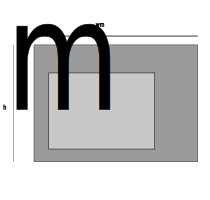
\includegraphics[width=0.5\textwidth]{./window-inkscape.png}
    \caption{Physimos window}
    \label{fig:mesh1}
\end{figure}

\LaTeXe.

\subsection{Coordinate Systems}

% TABLE
\begin{center}
% \begin{tabular}[t]{ | m{5em} | m{1cm}| m{1cm} | }
% \begin{tabular}[b]{ | m{5em} || m{2cm} | m{1cm} | } 

% \renewcommand{\arraystretch}{2.0} % vertical padding
% % \arraystretch{1}
% % \sas
% \setlength{\tabcolsep}{2.0em} % horizontal padding
% \setlength{\extrarowheight}{6pt}



% \renewcommand{\arraystretch}{2.0} % vertical padding
\setlength{\tabcolsep}{1.5em} % horizontal padding

    % \vspace*{10}z
\begin{tabular}{| c  c  c  c |}
    
    \hline
    Name & Symbol & Unit & $Matrix$ \\ 
    \hline
    \hline


    &   &   &  \\
    Input & i & \textit{sc} &  
    % \renewcommand{\arraystretch}{2.0} % vertical padding
    \( p_{x} = M_{i/x} p_i \) 
    \\


    &   &   &  \\ 
    Sanity & s & \textit{sc} &   $ M_{i/s} = 
                            \begin{pmatrix}
                            1 & 0 & 0 \\
                            0 & -1 & h_w \\
                            0 & 0 & 1 
                            \end{pmatrix}$
    \\ 


    &   &   &  \\ 
    Normalized & n & nn & \( M_{s/n} = 
                            \begin{pmatrix}
                            \frac{1}{w_w} & 0  \\
                            0 & \frac{1}{h_w} \\
                            \end{pmatrix} \) 
    \\ 


    &   &   &  \\ 
    Pixels & p & px &       %\renewcommand{\arraystretch}{2.0} 
                            \(    M_{s/p} = 
                            \begin{pmatrix}
                            CS_x & 0  \\
                            0 & CS_y \\
                            \end{pmatrix}\) 
    \\ 


    &   &   &  \\
    Millimeters & m & mm &      % \renewcommand{\arraystretch}{2.0} 
                                \(   M_{p/m} = 
                                \begin{pmatrix}
                                (\frac{dm}{dp})_x & 0  \\
                                0 & (\frac{dm}{dp})_y \\
                                \end{pmatrix}\)  
    \\ 


    &   &   &  \\ 
    \hline

\end{tabular}
\end{center}

\setlength{\tabcolsep}{0.0em} % horizontal padding

where: 
\begin{description}
    \item[$w_w$] = Window Width
    \item[$h_w$] = Window Height
    \item[$CS$]  = Content Scale 
    \item[$\frac{dm}{dp}$] = millimeters per pixel
\end{description}


\renewcommand{\arraystretch}{1.0} % Increase vertical spacing
\newcommand{\fixedrow}[1]{\rule{0pt}{3em}#1}

\end{document}

